\documentclass[11pt]{amsart}
\usepackage{geometry}                % See geometry.pdf to learn the layout options. There are lots.
\geometry{letterpaper}                   % ... or a4paper or a5paper or ... 
%\geometry{landscape}                % Activate for for rotated page geometry
%\usepackage[parfill]{parskip}    % Activate to begin paragraphs with an empty line rather than an indent
\usepackage{graphicx}


\usepackage{pstricks}


\usepackage{amssymb}
\usepackage{epstopdf}
\usepackage{hyperref}
\DeclareGraphicsRule{.tif}{png}{.png}{`convert #1 `dirname #1`/`basename #1 .tif`.png}

\title{Brief Article}
\author{The Author}
%\date{}                                           % Activate to display a given date or no date

\begin{document}
\maketitle
%\section{}
%\subsection{}

\section{Introduction}
We write a brief paper meant to support \href{http://www.mhpc.it/}{MHPC} 
lectures on scientific programming environment. The goal of this classes 
is to provide students scientific programming tools to develop scientific applications. 
The author is an engineer, with a Ph.D. in numerical analysis and hopefully these brief 
notes will hold the best habits of these two education paths. Achieving my goal no 
matter what, and in the most efficient way. Being passionate about sophisticated 
mathematical structures. Finite Elements is method that allows me to express my passion 
about mathematics, and meanwhile teach best programming practices. I apologise 
I can't teach programming something that does not stimulate my curiosity.

\section{Strong Problem}
Scientists solve problems. Among the pletora of existing problems 
we need to pick one, simple enough to be solved during te time dedicated to a single 
class, and sophisticated enough to be representative for more sophisticated ones. 
The answer is the Poisson's problem,
modeling the diffusion of temperature in a body.

Given a domain $\Omega\subset \mathbb{R}^2$.
Find $u$ such that:
\[
\left\{
\begin{array}{ll}
-\Delta u = f & \mathrm{in}\ \Omega \\
u = 0  & \mathrm{on}\ \partial\Omega
\end{array}
\right.
\]
Just one remark:
\[
\Delta u = \partial_{xx} u + \partial_{yy} u,
\]
where $x$ and $y$ are the two coordinates in $\mathbb{R}^2$.

In other words, the Poisson's problem is asking for a type of solution 
that is characterised by having two continuous derivatives, in mathematical 
sense we ask for $u\in C^2$. \emph{It can be proved} that such a solution exists and 
is unique. It is also true that such a solution can be \emph{found} in simple and
specific cases. In the next section we explore an alternative strategy.

\section{Continous Weak Problem}
In the previous section we looked at the Poisson's problem and noticed that searching 
for its solution in a strong form requires looking for a $C^2$ solution. This requirement 
is that strong, that can only be fulfilled in simple cases. 
The Finite Element (Method) si not really a method, it is rather the art of looking 
for solutions in vector spaces simpler than the one needed by the strong form.

We understand that a key role is played by the space $V$ substituting 
the $C^2$ space. Assuming $V$ is continuous (has an infinite set of basis 
functions) the first idea is to project the problem onto this particular space. 
Mathematically this is written as:
\[
-\int_\Omega \Delta u\, v = \int_\Omega f\, v \quad \forall v \in V
\]
If the projection procedure in functional spaces looks cryptical,
we can compare it to the geometrical projection. Consider $u$ a vector 
and $V$ the $\mathbb{R}^2$ space. The projection of $u$ onto $V$ is:
\[
u = u_1 \cdot \mathbf{e}_1 + u_2 \cdot \mathbf{e}_2,
\]
being $\mathbf{e}_1$, $\mathbf{e}_2$ the basis vectors for $V = \mathbb{R}^2$.
The analogy here should be clear once we think that $\mathbf{e}_i$ play the 
same role as $v$.  

If we want to really get rid of the second derivatives in our problem we can 
integrate by parts:
\[
\int_\Omega \nabla u \cdot \nabla v - 
\int_{\partial \Omega} u \,\nabla v \cdot \mathbf{n} = \int_\Omega f\, v.
\]
The boundary integral calls for the boundary conditions to come into play. 
Homogenous boundary conditions require $u=0\ \mathrm{on}\ \partial\Omega$.
This requirement has a very simple meaning: ``we do not need to project our solution
on the boundary'', as consequence: $v=0\ \mathrm{on}\ \partial\Omega$.
%term looks more nasty than it actually is. 
%Nevertheless we have picked a problem simple enough to postpone the 
%discussion on boundary conditions. On the boundary integral we have just
%the same flux term that we asked to be zero at the boundary, meaning, our 
%integral goes to zero.
We are left with:
\[
\int_\Omega \nabla u \cdot \nabla v = \int_\Omega f\, v.
\]

For simplicity, we look for $u$ in the very same space as $v$. 
Notice that this is a choice that works pretty well in this case, but
remember, Finite Elements is an art, not a method. This choice 
is arbitrary and there are cases in which this choice fails. 
The weak formulation 
of our original problem, looks like:

Find $u\in V$, such that:
\[
\int_\Omega \nabla u \cdot \nabla v = \int_\Omega f\, v, \quad \forall v \in V.
\]

The relation between the weak problem and the strong one 
is clarified by the Lax-Milgram theorem. This proofs 
that the weak form is equivalent to the strong one, meaning 
we can approximate the continuous weak problem to get the solution 
of the strong one. We conclude this section recalling that:
\[
\int_\Omega \nabla u \cdot \nabla v = \int_\Omega 
\left(
\begin{array}{c}
\partial_x u\\
\partial_y u\\
\end{array}
\right) \cdot
\left(
\begin{array}{c}
\partial_x v\\
\partial_y v\\
\end{array}
\right) = 
\int_\Omega \left(
\partial_x u\, \partial_x v + 
\partial_y u\, \partial_y v\right)
\]

\section{Discrete Weak Problem}

To plug the solution of the Poisson's problem inside a computer 
we need to discretise it. F. Brezzi has a very nice way to explain 
the relation between the continuous form and the discrete one:
``Just plug $h$ everywhere!''

Find $u_h\in V_h$, such that:
\[
\int_\Omega \nabla u_h \cdot \nabla v_h = \int_\Omega f\, v_h, \quad \forall v_h \in V_h.
\]

Of course the this graphical operation has some deep mathematical consequences
that are explained in a very elegant way by the C\'ea's Lemma. We express the 
meaning of this lemma with the sketch in Figure~\ref{fig:cea_lemma}. If $V_h$ is a two dimensional plane and $u$ a point in three dimensions. The distance between $u$ and $u_h$ is the minimal among the all possible distances 
between $u$ and any $v_h$.
\begin{figure}[h]
\centering
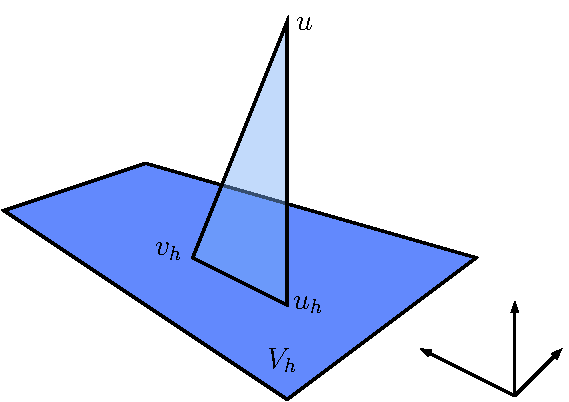
\includegraphics[scale=1]{cea_lemma-pics.pdf}
\caption{We represent in a three dimensional sketch the meaning of the C\'ea's Lemma.
If $V_h$ is a two dimensional plane and $u$ a point in three dimensions. The distance between $u$ and $u_h$ is the minimal among the all possible distances 
between $u$ and any $v_h$.}
\label{fig:cea_lemma}
\end{figure}

\section{Computational Solution of the Discrete Problem}

The first step toward the discretisation of the problem, is the discretisation 
of the domain. In Figure~\ref{fig:mesh} we represent the domain $\Omega$ and its 
discretisation, namely the triangulation $\mathcal{T}_h$. In this lecture notes we are 
going to consider triangular elements and linear shape functions. 

\begin{figure}[h]
\centering
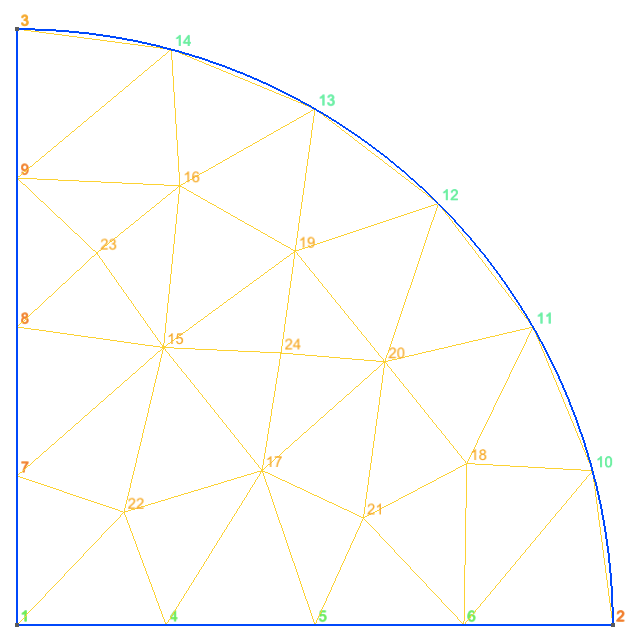
\includegraphics[scale=.3]{mesh.png}
\caption{A typical domain discretisation, in this case the original 
domain is a quarter of a circle.}
\label{fig:mesh}
\end{figure}

There are a pletora of possible basis functions that can be adopted on a discretised
domain. A subset of this pletora are defined on triangles, and among these we pick 
continuous linear functions, namely called $P_1$. Mathematically we can define the 
vector space $V_h$:
\[
V_h = \{\phi \in H^1_0{\Omega} : \phi|_K \in P_1(K) \forall K\in \mathcal{T}_h\}.
\]
$H^1_0(\Omega)$ is an Hilbert space, and $\phi$ is the collection of our basis 
functions, $K$ denotes the single triangle. We agree with the reader that this 
expression can be cryptic. In Figure~\ref{fig:local} we 
sketched the three linear basis functions on a triangle. The reader should notice 
that the $i$-th basis function is one on the $i$-th vertex and zero on the others. 
The three points are linearly connected in space. The linear functions are connected at 
each vertex forming a sort of tent. Figure~\ref{fig:mesh} highlights the global 
numbering of the vertices. Recall that in our problem $u_h\in V_h$, meaning that on 
every single element:
\[
u_h(x,y) = \sum_{i = 1}^3 u^j \phi_j(x,y) 
\]

\begin{figure}[h]
\centering
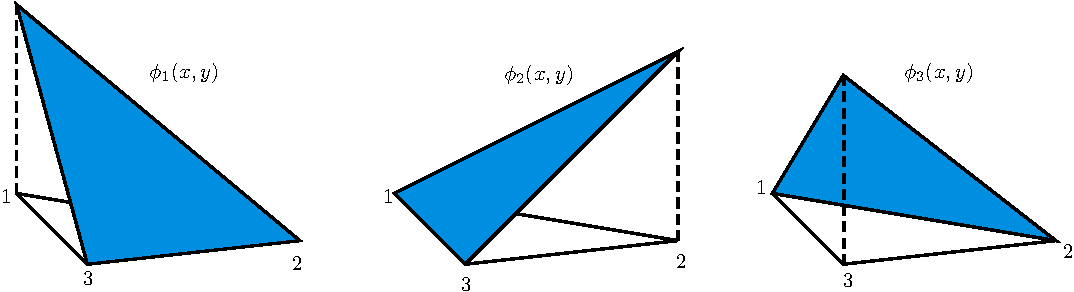
\includegraphics[scale=.8]{local_shape_funcs-pics.pdf}
\caption{Local linear shape functions on a triangular element.}
\label{fig:local}
\end{figure}

Figure~\ref{fig:tent} explains how the local basis functions are connected 
releasing the continuity of the solution space. 

\begin{figure}[h]
\centering
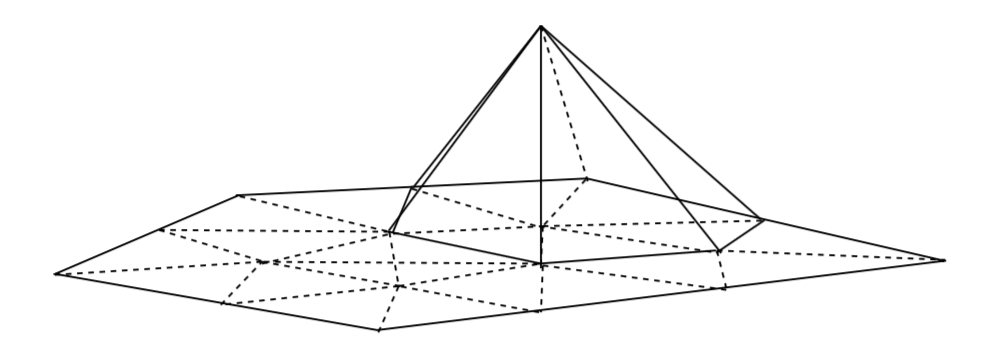
\includegraphics[scale=.4]{tent.png}
\caption{Global shape function on a domain. We can notice how the 
interelement continuity is achieved.}
\label{fig:tent}
\end{figure}

The last ingredient to establish an automatic strategy to solve our problem is 
to numerically compute an integral. 
Techniques that perform this task are called quadrature formulas. Among 
these, one that is particular suited for our linear case is the trapezoidal rule:
\[
\int_K \psi(x,y) \approx \mathrm{area}(K) \frac{1}{3}\sum_{q=1}^3\psi(x_q,y_q)
\]
where $\psi(x_q,y_q)$ is the integrand evaluated at the $q$-th quadrature point.

Now all the tools are in place, let's substitute in the left hand side (the most 
tricky one):
\[
\begin{split}
\int_\Omega \left(
\partial_x u\, \partial_x v + 
\partial_y u\, \partial_y v\right)\quad \forall v_h = \\
& \quad \sum_K \int_K \left(
\partial_x u\, \partial_x v + 
\partial_y u\, \partial_y v\right)\quad \forall v_h = \\
& \quad \sum_K \int_K \left(
\partial_x u\, \partial_x \phi_i + 
\partial_y u\, \partial_y \phi_i \right)\quad \forall i = \\
& \quad \sum_K \underbrace{\sum_j u^j  \int_K \left(
\partial_x \phi_j\, \partial_x \phi_i + 
\partial_y \phi_j\, \partial_y \phi_i \right)\quad \forall i}_{a_{ij} \, u^j}
\end{split}
\]
Easy enough the last step in our derivation can be expressed in matrix form as:
\[
\sum_K a_{ij} u^j.
\]
\[
a_{ij} u^j = 
\left(
\begin{array}{ccc}
\int_\Omega \left(
\partial_x \phi_1\, \partial_x \phi_1 + 
\partial_y \phi_1\, \partial_y \phi_1 \right) & 
\int_\Omega \left(
\partial_x \phi_2\, \partial_x \phi_1 + 
\partial_y \phi_2\, \partial_y \phi_1 \right) & 
\int_\Omega \left(
\partial_x \phi_3\, \partial_x \phi_1 + 
\partial_y \phi_3\, \partial_y \phi_1 \right)
\\
\int_\Omega \left(
\partial_x \phi_1\, \partial_x \phi_2 + 
\partial_y \phi_1\, \partial_y \phi_2 \right) & 
\int_\Omega \left(
\partial_x \phi_2\, \partial_x \phi_2 + 
\partial_y \phi_2\, \partial_y \phi_2 \right) & 
\int_\Omega \left(
\partial_x \phi_3\, \partial_x \phi_2 + 
\partial_y \phi_3\, \partial_y \phi_2 \right)\\
\int_\Omega \left(
\partial_x \phi_1\, \partial_x \phi_3 + 
\partial_y \phi_1\, \partial_y \phi_3 \right) & 
\int_\Omega \left(
\partial_x \phi_2\, \partial_x \phi_3 + 
\partial_y \phi_2\, \partial_y \phi_3 \right) & 
\int_\Omega \left(
\partial_x \phi_3\, \partial_x \phi_3 + 
\partial_y \phi_3\, \partial_y \phi_3 \right)
\end{array}
\right)
\]
$a_{ij}$ is called the local system matrix. It can be evaluated using the 
trapezoidal roule:
\[
\begin{split}
a_{ij} & = \frac{\mathrm{area}(K)}{3}\sum_{q=1}^3 \left(
\partial_x \phi_j\, \partial_x \phi_i + 
\partial_y \phi_j\, \partial_y \phi_i\right) = \\
& = \mathrm{area}(K)\left(
\partial_x \phi_j\, \partial_x \phi_i + 
\partial_y \phi_j\, \partial_y \phi_i\right) = \\
& = \mathrm{area}(K)\left(\left(
\begin{array}{c}
\partial_x \phi_1\\
\partial_x \phi_2\\
\partial_x \phi_3
\end{array}\right)
\left(
\begin{array}{ccc}
\partial_x \phi_1&
\partial_x \phi_2&
\partial_x \phi_3
\end{array}
\right)+
\left(
\begin{array}{c}
\partial_y \phi_1\\
\partial_y \phi_2\\
\partial_y \phi_3
\end{array}\right)
\left(
\begin{array}{ccc}
\partial_y \phi_1&
\partial_y \phi_2&
\partial_y \phi_3
\end{array}
\right)
\right)
\end{split}
\]
notice that derivatives of liner functions are constant.
The same procedure applies to the right and side:
\[
\tilde f_i = 
\frac{\mathrm{area}(K)}{3}\sum_{q=1}^3 \left(
f(x_q,y_q)\, \phi_i(x_q,y_q)\right)
\]
\[
\begin{split}
\tilde f_i = & 
\frac{\mathrm{area}(K)}{3} \left(
\begin{array}{c}
f(x_1,y_1)\, \phi_1(x_1,y_1) + f(x_2,y_2)\, \phi_1(x_2,y_2) + f(x_3,y_3)\, \phi_1(x_3,y_3)\\
f(x_1,y_1)\, \phi_2(x_1,y_1) + f(x_2,y_2)\, \phi_2(x_2,y_2) + f(x_3,y_3)\, \phi_2(x_3,y_3)\\
f(x_1,y_1)\, \phi_3(x_1,y_1) + f(x_2,y_2)\, \phi_3(x_2,y_2) + f(x_3,y_3)\, \phi_3(x_3,y_3)
\end{array}
\right)\\
&=
\frac{\mathrm{area}(K)}{3} \left(
\begin{array}{c}
f(x_1,y_1)\, 1 + f(x_2,y_2)\, 0 + f(x_3,y_3)\, 0\\
f(x_1,y_1)\, 0 + f(x_2,y_2)\, 1 + f(x_3,y_3)\, 0\\
f(x_1,y_1)\, 0 + f(x_2,y_2)\, 0 + f(x_3,y_3)\, 1
\end{array}
\right)\\
& =
\frac{\mathrm{area}(K)}{3} \left(
\begin{array}{c}
f(x_1,y_1)\\
f(x_2,y_2)\\
f(x_3,y_3)
\end{array}
\right)
\end{split}
\]
Figure~\ref{fig:assembly} should be explicative on how to account for local 
contributions in the global matrix. The final problem reduces to a linear system solution:
\[
A\, u^j = f_i.
\]
\begin{figure}[h]
\centering
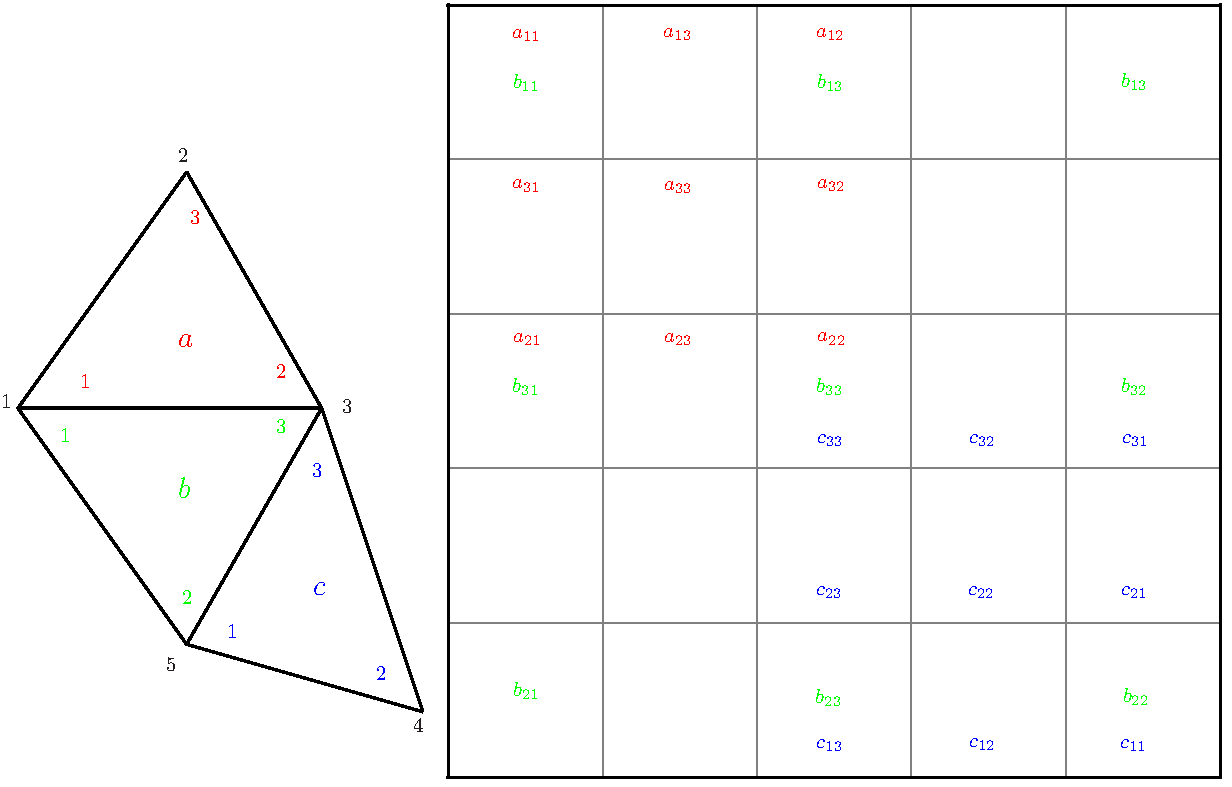
\includegraphics[scale=.8]{assembly-pics.pdf}
\caption{The assembly explained in one picture. On the left an example 
mesh. On the right, the grid represents the global matrix. Highlighted inside the 
grid the local contributions $a_{ij}$, $b_{ij}$, $c_{ij}$.}
\label{fig:assembly}
\end{figure}

\section{Homogeneous Boundary Conditions}
\[
\left(
\begin{array}{ccccc}
A_{11} & A_{12} & A_{13} & A_{14} & A_{15} \\
A_{21} & A_{22} & A_{23} & A_{24} & A_{25} \\ 
A_{31} & A_{32} & A_{33} & A_{34} & A_{35} \\ 
A_{41} & A_{42} & A_{43} & A_{44} & A_{45} \\ 
A_{51} & A_{52} & A_{53} & A_{54} & A_{55} \\ 
\end{array}
\right)
\left(
\begin{array}{c}
u^1\\
u^2\\
u^3\\
u^4\\
u^5\\
\end{array}
\right)
= 
\left(
\begin{array}{c}
f_1\\
f_2\\
f_3\\
f_4\\
f_5\\
\end{array}
\right)
\]
Say that nodes 2 and 4 belong to the boundary:
\[
\left(
\begin{array}{ccccc}
A_{11} & A_{12} & A_{13} & A_{14} & A_{15} \\
0      & A_{22} & 0      & 0      & 0 \\ 
A_{31} & A_{32} & A_{33} & A_{34} & A_{35} \\ 
0 &  0 & 0      & A_{44} & 0 \\ 
A_{51} & A_{52} & A_{53} & A_{54} & A_{55} \\ 
\end{array}
\right)
\left(
\begin{array}{c}
u^1\\
u^2\\
u^3\\
u^4\\
u^5\\
\end{array}
\right)
= 
\left(
\begin{array}{c}
f_1\\
0\\
f_3\\
0\\
f_5\\
\end{array}
\right)
\]
\appendix
\section{Basis Functions}
\[
\phi(x,y) = a\, x + b\, y + c
\]
\begin{align*}
\phi_1(x_1,y_1)  & =  a\, x_1 + b\, y_1 + c  =  1 \\
\phi_1(x_2,y_2)  & =  a\, x_2 + b\, y_2 + c  =  0 \\
\phi_1(x_3,y_3)  & =  a\, x_3 + b\, y_3 + c  =  0 \\
\end{align*}
\begin{align*}
  a\, x_1 + b\, y_1 + c  =  1 \\
  a\, x_2 + b\, y_2 + c  =  0 \\
  a\, x_3 + b\, y_3 + c  =  0 \\
\end{align*}
\[
\left(
\begin{array}{ccc}
x_1 & y_1 & 1 \\
x_2 & y_2 & 1 \\
x_3 & y_3 & 1 
\end{array}
\right)
\left(
\begin{array}{c}
a\\
b\\
c\\
\end{array}
\right) =
\left(
\begin{array}{c}
1\\
0\\
0\\
\end{array}
\right)
\]


\begin{align*}
\phi_2(x_1,y_1)  & =  a\, x_1 + b\, y_1 + c  =  0 \\
\phi_2(x_2,y_2)  & =  a\, x_2 + b\, y_2 + c  =  1 \\
\phi_2(x_3,y_3)  & =  a\, x_3 + b\, y_3 + c  =  0 \\
\end{align*}
\begin{align*}
\phi_3(x_1,y_1)  & =  a\, x_1 + b\, y_1 + c  =  0 \\
\phi_3(x_2,y_2)  & =  a\, x_2 + b\, y_2 + c  =  0 \\
\phi_3(x_3,y_3)  & =  a\, x_3 + b\, y_3 + c  =  1 \\
\end{align*}
\end{document}  